\documentclass[table]{article}

% Idioma: español
\usepackage[spanish,es-lcroman]{babel} % Características del idioma
\usepackage[utf8]{inputenc} % Acentos


% Aspecto de página
\usepackage[a4paper,vmargin=1in]{geometry} % Márgenes
\usepackage{fancyhdr} % Headers
\usepackage{parskip} % Espacio entre párrafos
\usepackage{microtype} % Kerning y mejoras tipográficas
\usepackage{pagecolor} % Color de fondo
\usepackage{everypage} % \AddThispageHook {\tikz[remember picture,overlay] ... }

% Columnas y tablas
\usepackage{multicol}

\usepackage{multirow}
\usepackage{tabularx}
\usepackage{tabu}
\usepackage{diagbox} % Dividir una celda de un tabular
\def\arraystretch{1}

% Imágenes
\usepackage{graphicx}
\usepackage{wrapfig}
\usepackage{caption}
\graphicspath{{img/}}

% Símbolos
\usepackage{mathtools} % \text, \overset, \underset
\usepackage{amssymb} % \mathbb
\usepackage{upgreek} % \uptheta
\usepackage{amsthm} % QED
\usepackage{marvosym} % \EUR

% Formato
\usepackage{xcolor}
\usepackage{soul} % \so, \st, \hl
\usepackage{cancel} % \cancel, \bcancel, \xcancel, \cancelto
\newcommand*\canceling[2][thin]{\tikz[baseline] \node [strike out,draw,anchor=text,inner sep=0pt,text=black,#1]{#2};}

% Listas
\usepackage{enumerate} % Numeración de listas
\usepackage{outlines} % \0 \1 \2 \3 \4
% Dibujos y gráficas
\usepackage{tikz} 
\usepackage{pgfplots}
\usetikzlibrary{shapes,arrows,decorations.markings,shapes.misc,shapes.geometric,calc,pgfplots.groupplots}
\pgfplotsset{compat=1.13}

% Índices y títulos
\addto\captionsspanish{\renewcommand{\contentsname}{Índice}}
\usepackage{titlesec} % Formato de títulos
%\usepackage{minitoc} % Índices de secciones
\usepackage{hyperref} % Links
\hypersetup{colorlinks}

% Otros
\usepackage[spanish,colorinlistoftodos,obeyDraft]{todonotes} % ToDo
\usepackage{pdfpages} % Incluir PDFs
\usepackage{qrcode} % QR
\usepackage{chemfig} % Química
\usepackage{wasysym} % Notas musicales

\usepackage[acronym]{glossaries} % Siglas y glosario
\usepackage{acronym} % Acrónimos


% Código
\usepackage{listingsutf8}
\lstset{
	inputencoding=utf8,
	extendedchars=true,
	literate=%
	{á}{{\'a}}1
	{é}{{\'e}}1
	{í}{{\'i}}1
	{ó}{{\'o}}1
	{ú}{{\'u}}1
	{Á}{{\'A}}1
	{É}{{\'E}}1
	{Í}{{\'I}}1
	{Ó}{{\'O}}1
	{Ú}{{\'U}}1
	{ñ}{{\~n}}1
	{Ñ}{{\~N}}1
	{¿}{{<}}1
	{¡}{{>}}1
}

% Apéndices
\newcommand{\apendices}
{\section*{Apéndices}%
	\addcontentsline{toc}{section}{Apéndices}
	\setcounter{section}{0}%
	\setcounter{subsection}{0}%
	\renewcommand\thesection{\Alph{section}}%
}

\title{Dossier grupo C+++}
\author{}
\date{}


\begin{document}
	
	
%	\maketitle
%	
%	\begin{abstract}\end{abstract}
%	
%	\tableofcontents
%	
%	\section{}



\definecolor{mygreen}{rgb}{0,0.6,0}
\definecolor{mypurple}{rgb}{0.7,0.3,0.7}
\lstset{
	language=C++,
%	backgroundcolor=\color{white},
%	frame=single,
	%
	basicstyle=\tt,
	commentstyle=\itshape\color{mygreen},
	keywordstyle=\color{magenta},
	identifierstyle=\color{cyan},
	stringstyle=\color{mypurple},
	emph={int,char,double,float,unsigned,void,bool},	
	emphstyle={\color{blue}},
	showstringspaces=false,
	columns=flexible,
	%
	numbers=none,
	numberstyle=\color{gray},
	firstnumber = 1,
	stepnumber=2,
	tabsize =2,
	escapechar=¬
}
%\lstset{
%	language=C++,
%	backgroundcolor=\color{pink},
%	frame=trBL,
%	%
%	basicstyle=\tt\color{white},
%}

\vspace{-10cm}
\maketitle

\vspace*{-1cm}
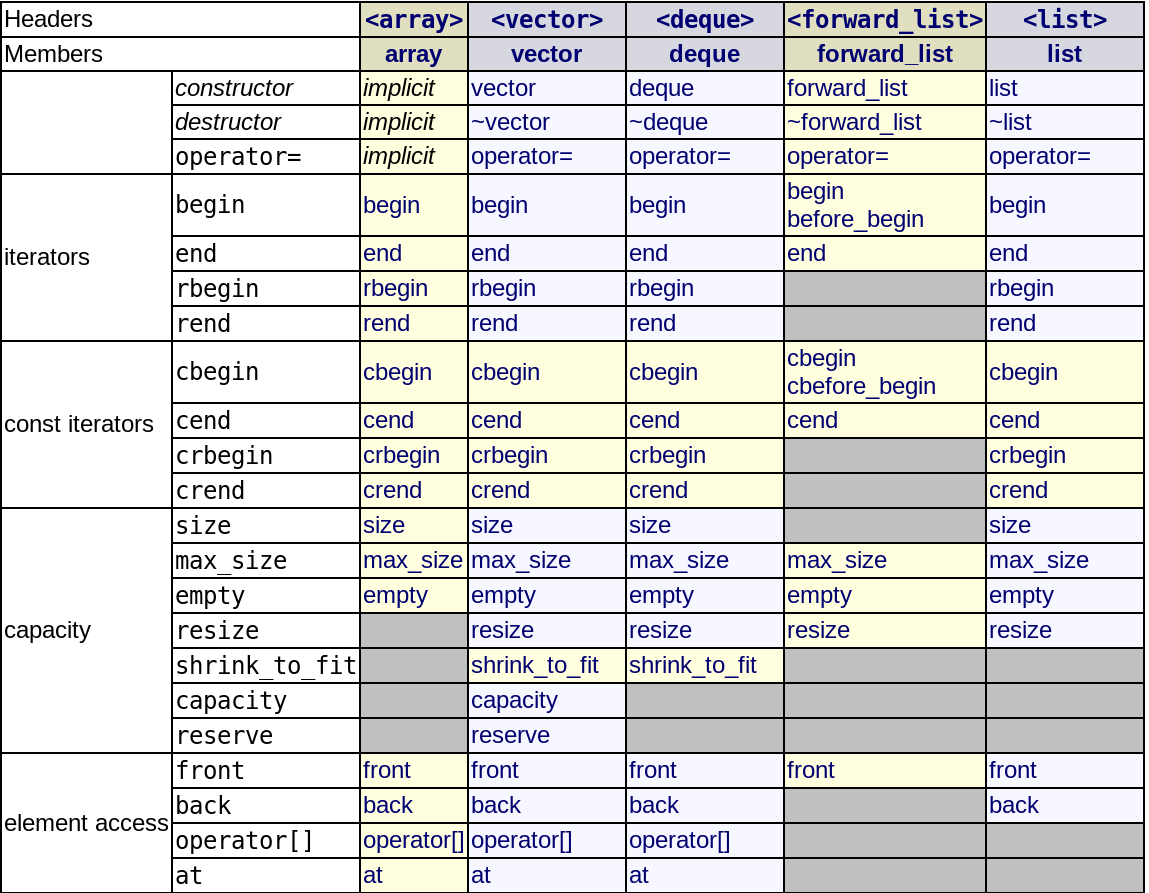
\includegraphics[width=\textwidth]{1.png}
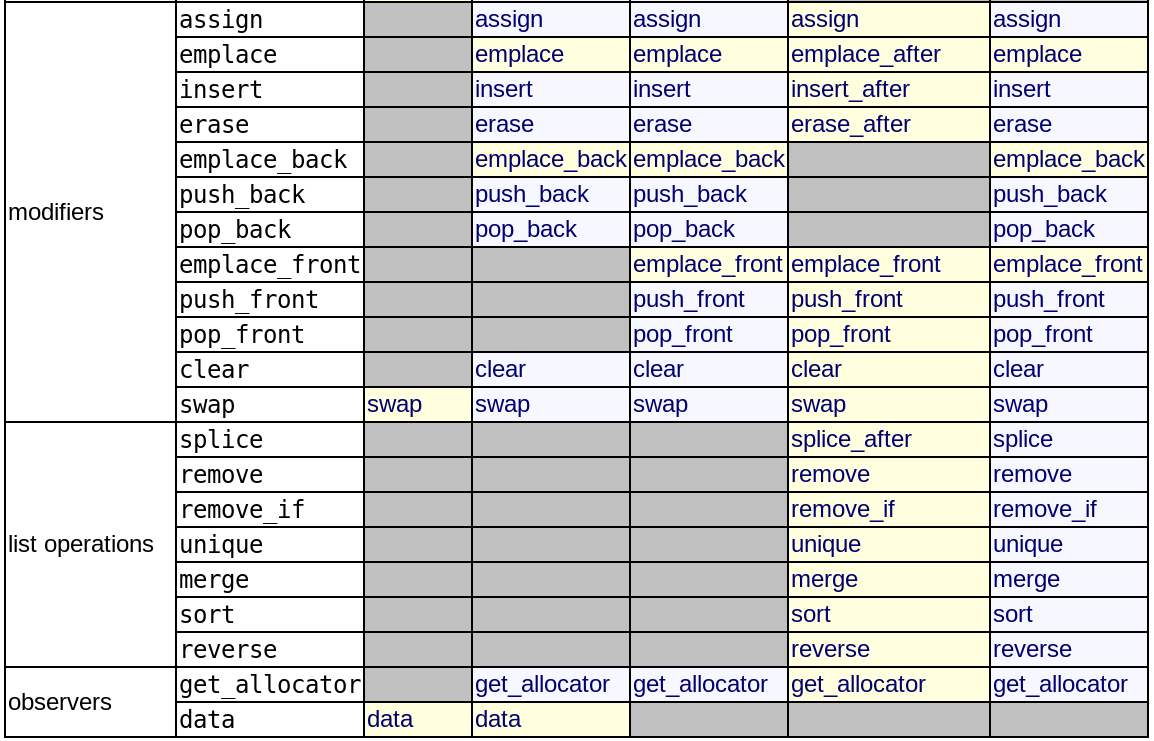
\includegraphics[width=\textwidth]{2.png}\\

\vspace*{-1cm}
\hspace*{-2.5cm}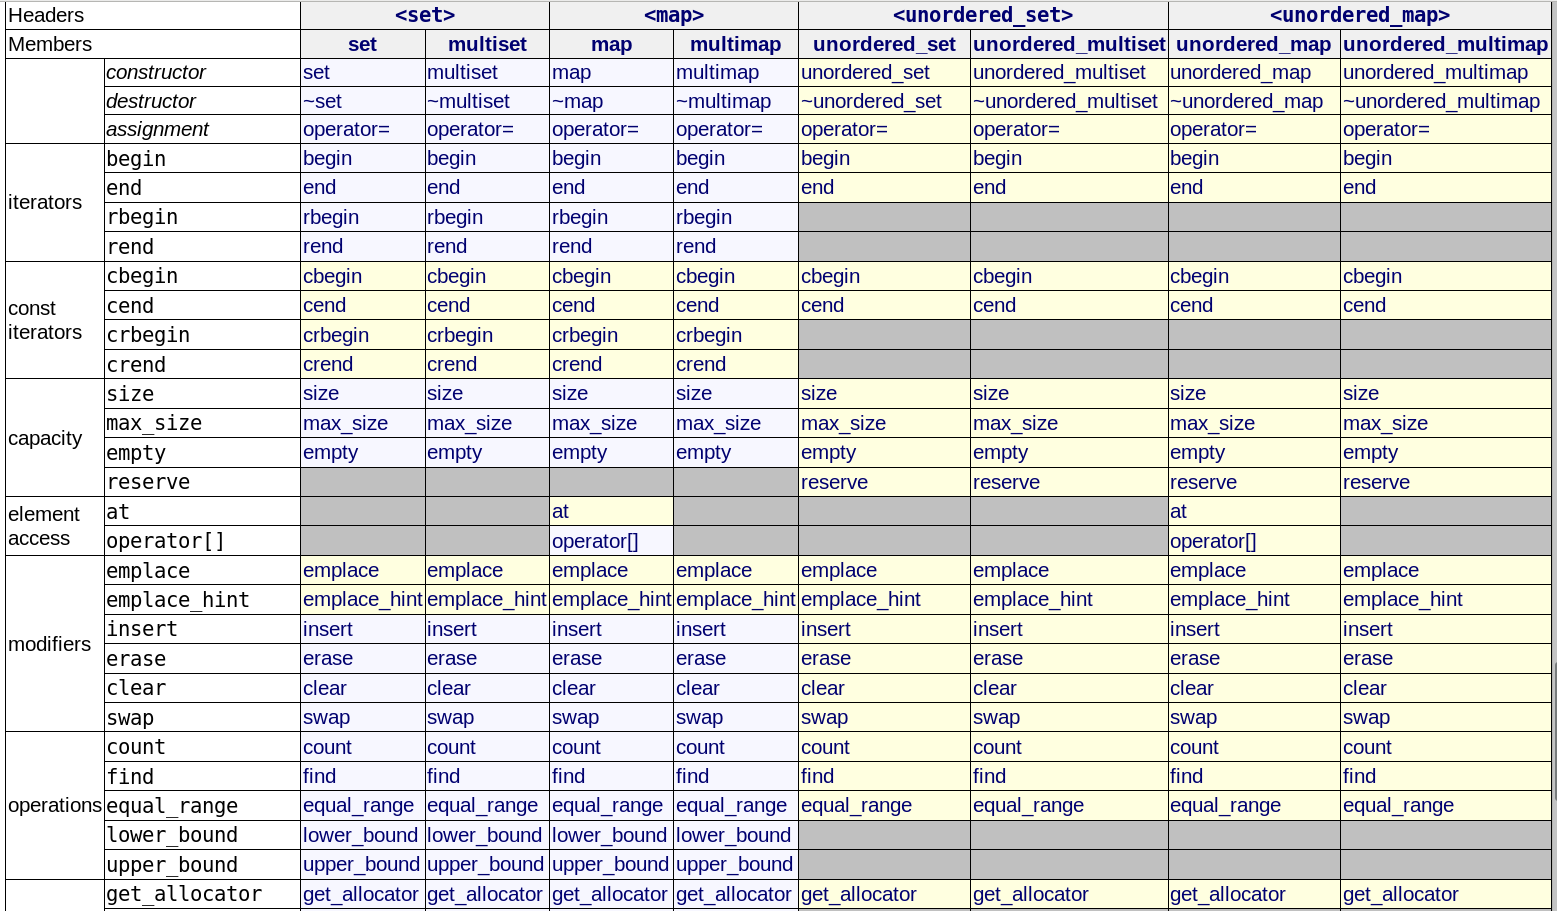
\includegraphics[width=0.95\paperwidth]{3.png}\\

\textbf{stack:} empty, size, top, push, emplace, pop, swap

\textbf{queue:} empty, size, front, back, push, emplace, pop, swap

\textbf{priority\_queue:} empty, size, top, push, emplace, pop, swap\\

memset(char[] str,'-',6);

cstdlib : atoi (char[] to int), qsort, bsearch

cstdio : printf, scanf, getc, putc, eof

cctype : tolower, toupper, islower, isupper, ispunct

iomanip : setfill, setw, setprecision

cmath : exp, log, pow, sqrt, cbrt, ceil, floor, round, abs

algorithm : sort, merge, copy, move, min, max, reverse, rotate

utility : pair, swap, less

climits : INT\_MIN, INT\_MAX, LONG\_, LLONG\_
	
	\pagebreak
	\normalsize
	\begin{multicols}{2}
	\subsection*{Non-modifying sequence ops:}
	
	\textbf{all\_of}\\
	Test condition on all elements in range
	
	\textbf{any\_of}\\
	Test if any element in range fulfills condition
	
	\textbf{none\_of}\\
	Test if no elements fulfill condition
	
	\textbf{for\_each}\\
	Apply function to range
	
	\textbf{find}\\
	Find value in range
	
	\textbf{find\_if}\\
	Find element in range
	
	\textbf{find\_if\_not}\\
	Find element in range (negative condition)
	
	\textbf{find\_end}\\
	Find last subsequence in range
	
	\textbf{find\_first\_of}\\
	Find element from set in range
	
	\textbf{adjacent\_find}\\
	Find equal adjacent elements in range
	
	\textbf{count}\\
	Count appearances of value in range
	
	\textbf{count\_if}\\
	Return number of elements in range satisfying condition
	
	\textbf{mismatch}\\
	Return first position where two ranges differ
	
	\textbf{equal}\\
	Test whether the elements in two ranges are equal
	
	\textbf{is\_permutation}\\
	Test whether range is permutation of another
	
	\textbf{search}\\
	Search range for subsequence
	
	\textbf{search\_n}\\
	Search range for elements
	
	\subsection*{Modifying sequence operations:}
	
	\textbf{copy}\\
	Copy range of elements
	
	\textbf{copy\_if}\\
	Copy certain elements of range
	
	\textbf{copy\_backward}\\
	Copy range of elements backward
	
	\textbf{move}\\
	Move range of elements
	
	\textbf{move\_backward}\\
	Move range of elements backward
	
	\textbf{swap}\\
	Exchange values of two objects
	
	\textbf{swap\_ranges}\\
	Exchange values of two ranges
	
	\textbf{iter\_swap}\\
	Exchange values of objects pointed to by two iterators
	
	\textbf{transform}\\
	Transform range
	
	\textbf{replace}\\
	Replace value in range
	
	\textbf{replace\_if}\\
	Replace values in range
	
	\textbf{fill}\\
	Fill range with value
	
	\textbf{remove}\\
	Remove value from range
	
	\textbf{remove\_if}\\
	Remove elements from range
	
	\textbf{unique}\\
	Remove consecutive duplicates in range
	
	\textbf{reverse}\\
	Reverse range
	
	\textbf{rotate}\\
	Rotate left the elements in range
	
	\subsection*{Partitions:}
	
	\textbf{is\_partitioned}\\
	Test whether range is partitioned
	
	\textbf{partition}\\
	Partition range in two
	
	\textbf{stable\_partition}\\
	Partition range in two - stable ordering
	
	\textbf{partition\_point}\\
	Get partition point
	
	\subsection*{Sorting:}
	
	\textbf{sort}\\
	Sort elements in range
	
	\textbf{stable\_sort}\\
	Sort elements preserving order of equivalents
	
	\textbf{partial\_sort}\\
	Partially sort elements in range
	
	\textbf{is\_sorted}\\
	Check whether range is sorted
	
	\textbf{is\_sorted\_until}\\
	Find first unsorted element in range
	
	\textbf{nth\_element}\\
	Sort element in range
	
	\subsection*{Binary search:}
	
	\textbf{lower\_bound}\\
	Return iterator to lower bound
	
	\textbf{upper\_bound}\\
	Return iterator to upper bound
	
	\textbf{equal\_range}\\
	Get subrange of equal elements
	
	\textbf{binary\_search}\\
	Test if value exists in sorted sequence
	
	\subsection*{Merge:}
	
	\textbf{merge}\\
	Merge sorted ranges
	
	\textbf{inplace\_merge}\\
	Merge consecutive sorted ranges
	
	\textbf{includes}\\
	Test whether sorted range includes another sorted range
	
	\textbf{set\_union}\\
	Union of two sorted ranges
	
	\textbf{set\_intersection}\\
	Intersection of two sorted ranges
	
	\textbf{set\_difference}\\
	Difference of two sorted ranges
	
	\textbf{set\_symmetric\_difference}\\
	Symmetric difference of two sorted ranges
	
	\subsection*{Min/max:}
	
	\textbf{min}\\
	Return the smallest
	
	\textbf{max}\\
	Return the largest
	
	\textbf{minmax}\\
	Return smallest and largest elements
	
	\textbf{min\_element}\\
	Return smallest element in range
	
	\textbf{max\_element}\\
	Return largest element in range
	
	\textbf{minmax\_element}\\
	Return smallest and largest elements in range
	
	\subsection*{Other:}
	
	\textbf{next\_permutation}\\
	Transform range to next permutation
	
	\textbf{prev\_permutation}\\
	Transform range to previous permutation
	
	\end{multicols}
	\pagebreak

	\normalsize\lstinputlisting[language=C++]{dossier.cpp}

\end{document}
